\documentclass[letterpaper, journal, twocolumn]{IEEEtran}
\usepackage{amsmath,amssymb,amsfonts}
\usepackage{graphicx}
\usepackage{booktabs}
\usepackage{cite}
\usepackage{url}
\usepackage{tikz}
\usetikzlibrary{arrows.meta,positioning,calc}
\usepackage{microtype}
\usepackage{balance}
\usepackage{array}
\usepackage{algorithm}
\usepackage{algpseudocode}

\graphicspath{{../fig/}}

\begin{document}

\title{Real-Time Marginal Ambiguity Covariance for\\
Tightly Coupled GNSS--Visual--Inertial Factor Graphs}

\author{Anonymous Authors
\thanks{Manuscript prepared for IEEE Robotics and Automation Letters (RAL).
Numerical claims are traced to logged per-epoch benchmarks and
\texttt{results/research/paper\_repro/} where cited.
Ground truth is used only in post-hoc evaluation.}}

\maketitle

\begin{abstract}
Carrier-phase ambiguity resolution (AR) in tightly coupled GNSS/IMU/vision
estimators consumes a float ambiguity covariance $Q_{aa}$.
Open platforms often substitute a GNSS-only ``shadow'' covariance because
forming the joint sliding-window covariance online is considered too
expensive, discarding the IMU and visual information that tight coupling is
meant to provide.
We present an exact-in-window marginal
$Q_{aa}=[H_{\mathrm{active}}^{-1}]_{aa}$ obtained by two-stage sparse Schur
elimination over the active GNSS--IMU--vision window, including the
marginalization prior, with a numerical self-validation gate and shadow
fallback.
On 1\,787 open-sky AR epochs the method produces a validated covariance on
99.94\% of epochs, with 90.1\% achieving relative Frobenius error
$\|Q_{\mathrm{prop}}-Q_{\mathrm{Ceres}}\|_F/\|Q_{\mathrm{Ceres}}\|_F$ below
$10^{-3}$; among the remaining disagreements a trace proxy is larger
(conservative) in 171 of 177 cases and within $7.3\times10^{-4}$ in 6
near-ties.
Mean covariance query time is 28\,ms versus 812\,ms for Ceres
($\sim$29$\times$), with median 27\,ms, p95 49\,ms, p99 59\,ms, and 4.3\% of
epochs above a 50\,ms covariance budget (max 97.5\,ms).
End-to-end effects versus shadow AR are reported as secondary system impact;
an overconfident local-conditioning approximation is harmful.
Full matrix Loewner diagnostics and a Ceres end-to-end oracle are required to
support a stronger ``exact'' claim and are in progress
(Sec.~\ref{sec:limits}).
\end{abstract}

\begin{IEEEkeywords}
RTK, ambiguity resolution, factor graph, marginal covariance,
GNSS/IMU/vision, Schur complement
\end{IEEEkeywords}

%======================================================================
\section{Introduction}
\label{sec:intro}

Tightly coupled GNSS/IMU/vision estimators resolve carrier-phase integers
using a float ambiguity covariance fed to LAMBDA-type search and acceptance
tests.
In GICI-LIB~\cite{chi2023gici}, the open RTK/IMU/camera reference, AR
consumes a covariance from a parallel GNSS-only shadow estimator because a
full-graph query via \texttt{ceres::Covariance} is too slow online
(mean 812\,ms on our filled-window open-sky graphs; 99.6\% of epochs exceed
50\,ms).
The shadow path discards IMU and visual information at the moment AR needs it
most.

Cheaper alternatives that condition on neighboring states without forming the
Schur complement are fast but can be overconfident: on UrbanNav Deep, a
local-conditioning variant raised fix rate while degrading horizontal RMSE
from $2.77{\pm}0.44$\,m to $6.75{\pm}2.98$\,m.
AR therefore needs a covariance that is both \emph{consistent with the joint
window} and \emph{affordable every epoch}.

This paper focuses on that covariance problem.
We make three contributions:
\begin{enumerate}
\item An algorithm that extracts the exact-in-window marginal ambiguity
  covariance $Q_{aa}=[H_{\mathrm{active}}^{-1}]_{aa}$ by structure-exploiting
  two-stage elimination, without inverting the full information matrix and
  without dropping the marginalization prior.
\item A numerical self-validation gate with typed abstention and shadow
  fallback, so an unreliable factorization never feeds AR.
\item A covariance-level evaluation against shadow AR, local conditioning, and
  \texttt{ceres::Covariance}, with end-to-end system impact reported secondarily.
\end{enumerate}

The two evaluation questions are: (i)~does the proposed path reproduce the
Ceres ambiguity covariance (and, offline, Ceres-driven AR decisions)?
(ii)~by how much does it reduce cost relative to the estimator/AR cycle?
Trajectory RMSE is secondary and is not the headline claim.

%======================================================================
\section{Related Work}
\label{sec:related}

\paragraph{Integer estimation.}
ILS via LAMBDA~\cite{teunissen1995lambda} / MLAMBDA~\cite{chang2005mlambda},
ratio tests and FFRT~\cite{verhagen2013ffrt,euler1990ratio}, partial AR, and
bootstrapping success rates~$P_s$~\cite{teunissen1998success} are standard.
BIE~\cite{teunissen2003bie,odolinski2020bie} softens hard commits.
Our focus is the float covariance that those methods consume inside a
multi-sensor graph, not a new integer estimator.

\paragraph{GNSS/IMU/vision fusion.}
Tight VIO~\cite{qin2018vins,leutenegger2015okvis} and GNSS--VIO
systems~\cite{cao2022gvins,chi2023gici} optimize sliding-window factor graphs
with marginalization priors.
GICI-LIB's AR path uses a GNSS-only shadow covariance---the gap we close at
the covariance interface.

\paragraph{Covariance recovery in factor graphs.}
Marginal covariances are classical in Gauss--Newton estimation.
Sparse factorization and selected inversion recover subsets of
$H^{-1}$ without forming the full dense inverse~\cite{erisman1975sparse,li2008selected}.
Incremental smoothers (iSAM2 / Bayes tree) maintain square-root information
and can extract covariances from the clique
structure~\cite{kaess2012isam2,dellaert2017factor}.
Ceres exposes sparse-QR covariance queries~\cite{agarwal2023ceres} that are
exact for the linearized problem but costly on large live windows.
Our method is a domain-structured elimination for the ambiguity block of a
GNSS/IMU/vision RRR window: landmark Schur first, then dense reduction of the
remaining nuisance states, with an AR-oriented abstention policy.

\paragraph{Urban GNSS.}
NLOS/multipath mitigations include masks, robust losses, shadow
matching~\cite{groves2011shadow}, and 3DMA~\cite{ng2020_3dma,wen2021nlos}.
UrbanNav-HK~\cite{huang2020urbannav} provides Medium/Deep benchmarks.
We use these datasets to stress end-to-end AR under the proposed $Q_{aa}$; we
do not claim a new NLOS classifier.

%======================================================================
\section{Problem Formulation}
\label{sec:problem}

We consider a Ceres-based sliding-window RRR graph with double-differenced
GNSS residuals, IMU preintegration, reprojection factors, and a dense
marginalization prior.
Let $x$ collect active states and $H=\sum_r J_r^\top J_r$ the Gauss--Newton
information in minimal coordinates (Triggs-corrected Jacobians for robust
residuals), including the prior information $\Lambda$.
Partition $x=(a,\ell,n)$ into ambiguities $a$, landmarks $\ell$, and remaining
nuisance $n$ (poses, speed/bias, clocks, frequencies, extrinsics, prior-only
variables).

AR requires the marginal
\begin{equation}
\label{eq:qaa}
Q_{aa} = \bigl[H^{-1}\bigr]_{aa}.
\end{equation}
\texttt{ceres::Covariance} computes~\eqref{eq:qaa} at whole-problem sparse-QR
cost.
The shadow estimator replaces~\eqref{eq:qaa} with a GNSS-only approximation.
A local-conditioning shortcut drops the Schur term involving out-of-set
neighbors and is fast but can understate uncertainty.

\paragraph{Requirements.}
(R1)~Exactness in the active window: $Q_{aa}$ must equal the Ceres marginal up
to linearization and numerics.
(R2)~Real-time: cost bounded by window size, with a fallback when factorization
is unreliable.
(R3)~AR safety preference: when numerics disagree, prefer larger uncertainty
over silent overconfidence.

Fig.~\ref{fig:arch} places $Q_{aa}$ in the AR path.

\begin{figure}[!t]
\centering
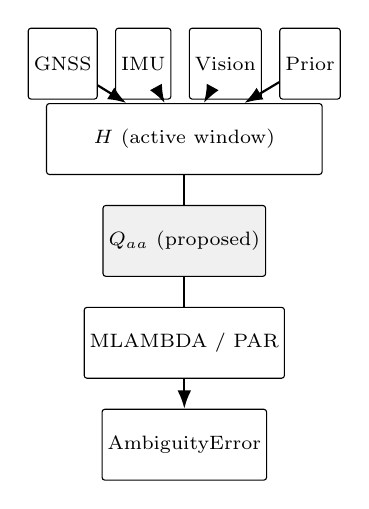
\begin{tikzpicture}[
  box/.style={draw, rounded corners=1pt, align=center, font=\scriptsize,
    inner sep=2pt, minimum height=0.9cm},
  arr/.style={-{Latex}, thick}]
\node[box] (gnss) {GNSS};
\node[box, right=0.22 of gnss] (imu) {IMU};
\node[box, right=0.22 of imu] (vis) {Vision};
\node[box, right=0.22 of vis] (prior) {Prior};
\node[box, below=0.5 of $(imu)!0.5!(vis)$, minimum width=3.5cm]
  (H) {$H$ (active window)};
\node[box, below=0.38 of H, fill=black!6] (Q) {$Q_{aa}$ (proposed)};
\node[box, below=0.38 of Q] (L) {MLAMBDA / PAR};
\node[box, below=0.38 of L] (fix) {AmbiguityError};
\foreach \a/\b in {gnss/H,imu/H,vis/H,prior/H}
  \draw[arr] (\a) -- (\b);
\draw[arr] (H) -- (Q) -- (L) -- (fix);
\end{tikzpicture}
\caption{RRR window and AR path. The shaded block is the proposed
exact-in-window marginal; the baseline uses a GNSS-only shadow covariance
instead.}
\label{fig:arch}
\end{figure}

%======================================================================
\section{Proposed Marginal Covariance Method}
\label{sec:method}

\paragraph{Assembly.}
We form $H$ from all active residuals plus the marginalization prior through a
read-only accessor exposing $\Lambda=J^\top J$ with per-block minimal offsets
(generic residual evaluation of the prior is avoided under live window growth).

\paragraph{Two-stage elimination.}
No residual couples an ambiguity to a landmark ($H_{a\ell}=0$; prior-touched
landmarks are promoted into $n$), so
\begin{equation}
H=\begin{bmatrix}
H_{aa} & H_{an} & 0 \\
H_{na} & H_{nn} & H_{n\ell} \\
0 & H_{\ell n} & H_{\ell\ell}
\end{bmatrix}.
\end{equation}
Stage~1 forms the landmark Schur update
\begin{equation}
\bar H_{nn}=H_{nn}-H_{n\ell}H_{\ell\ell}^{+}H_{\ell n}
\end{equation}
via independent $3\times3$ rank-truncated pseudo-inverses.
\emph{Exactness condition:} null modes of each $H_{ii}$ have zero coupling
rows in $H_{\ast i}$, so truncating those modes does not change the
$(a,n)$ marginal.
Stage~2 then yields the ambiguity marginal
\begin{equation}
\label{eq:qaa-schur}
Q_{aa}=\Bigl(H_{aa}-H_{an}\bar H_{nn}^{-1}H_{na}\Bigr)^{-1}
\end{equation}
by Jacobi-equilibrated dense LDLT on $\bar H_{nn}$ plus iterative refinement
(Fig.~\ref{fig:schur}, Alg.~\ref{alg:cov}).

\paragraph{Relation to standard covariance recovery.}
Ceres selected covariance~\cite{agarwal2023ceres} asks for the same blocks but
factors the \emph{whole} problem (sparse QR) each query.
Sparse selected inversion / Takahashi methods recover entries of $H^{-1}$ from
a global factorization~\cite{erisman1975sparse,li2008selected}; Bayes-tree
methods reuse incremental square-root information~\cite{kaess2012isam2}.
Our contribution is not a new linear-algebra primitive but a
\emph{domain-structured online path}: landmark blocks are eliminated at
$O(1)$ each, the remaining GNSS/IMU/extrinsic/prior nuisance is small enough
for dense reduction every AR epoch, the marginalization prior is included
through a read-only $\Lambda$ accessor, and a typed abstention prevents feeding
AR an untrusted $Q_{aa}$.
Complexity: $O(L)$ for $L$ landmarks ($3\times3$ each) plus
$O(n_n^3+n_a n_n^2)$ for nuisance size $n_n$ and ambiguity size $n_a$,
bounded by the sliding window.

\paragraph{Self-validation and fallback.}
After LDLT, a few refinement steps on the reduced system are accepted only if
the last increment's effect on the Schur complement is below the scale of the
smallest eigenvalue of the reduced nuisance block (no dataset-tuned
thresholds).
Abstention cases: non-finite assembly, failed factorization, failed gate, or
non-PD reduced ambiguity information.
On abstention the estimator returns the shadow covariance for that epoch.

\begin{algorithm}[!t]
\caption{Exact-in-window marginal ambiguity covariance}
\label{alg:cov}
\begin{algorithmic}[1]
\Require active residuals, prior $\Lambda$, ambiguity index set $a$
\State Assemble $H\leftarrow\sum_r J_r^\top J_r$ (Triggs) $+\Lambda$
\For{each landmark block $\ell$}
  \State Rank-truncated Schur-eliminate $\ell$ from $H$
\EndFor
\State Jacobi-equilibrate nuisance; LDLT factorize
\State Iterative refine; \textbf{if} gate fails \textbf{then} \Return shadow $Q$
\State \Return $Q_{aa}\leftarrow[H_{\mathrm{red}}^{-1}]_{aa}$
\end{algorithmic}
\end{algorithm}

\begin{figure}[!t]
\centering
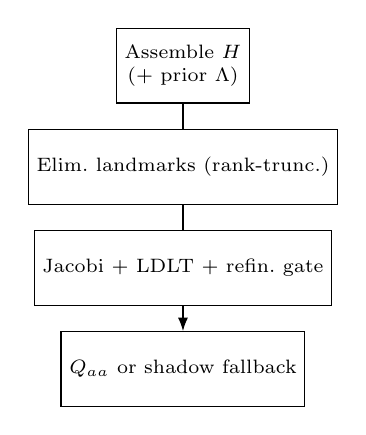
\begin{tikzpicture}[
  box/.style={draw, font=\scriptsize, align=center, inner sep=3pt,
    minimum height=0.95cm},
  arr/.style={-{Latex}}]
\node[box] (a) {Assemble $H$\\(+ prior $\Lambda$)};
\node[box, below=0.32 of a] (b) {Elim.\ landmarks (rank-trunc.)};
\node[box, below=0.32 of b] (c) {Jacobi + LDLT + refin.\ gate};
\node[box, below=0.32 of c] (d) {$Q_{aa}$ or shadow fallback};
\draw[arr] (a) -- (b) -- (c) -- (d);
\end{tikzpicture}
\caption{Two-stage elimination with abstention (F2).}
\label{fig:schur}
\end{figure}

The estimator is registered as an opt-in variant
(\texttt{rtk\_imu\_camera\_rrr\_va}); upstream defaults are unchanged.
File-mode UrbanNav configs disclose \texttt{max\_age}=35\,s (for 30\,s HKKT
base epochs) and \texttt{relative\_frequency}=0.01 (code default); neither was
tuned against UrbanNav ground truth.

%======================================================================
\section{Numerical Validation and Complexity}
\label{sec:numeric}

\paragraph{Reference.}
Per-AR-epoch comparison against \texttt{ceres::Covariance} on identical live
graphs (GICI-board~1.1, 1\,787 epochs), requesting the \emph{same} ambiguity
blocks (not a whole-state inverse straw man).
The primary match metric already logged online is the normalized Frobenius
error $\|Q_{\mathrm{prop}}-Q_{\mathrm{Ceres}}\|_F/\|Q_{\mathrm{Ceres}}\|_F$.
Trace comparisons are a secondary safety proxy only.
Loewner / directional diagnostics
($\min\mathrm{eig}(Q_{\mathrm{prop}}-Q_{\mathrm{Ceres}})$, generalized
eigenvalues of the pair) are instrumented in the benchmark path and must be
reported before a stronger exactness claim (Sec.~\ref{sec:limits}).

\paragraph{Accuracy.}
Table~\ref{tab:t1}: a validated covariance is produced on 99.94\% of epochs
(one abstention)---this is \emph{not} a 99.94\% match rate.
Of usable epochs, 90.1\% have Frobenius relative error $\le10^{-3}$.
Of 177 larger Frobenius disagreements, a trace proxy is larger in 171 cases
and within $7.3\times10^{-4}$ in 6 near-ties.
Larger trace does \emph{not} imply Loewner dominance in every direction.

\paragraph{Runtime.}
Table~\ref{tab:runtime} and Fig.~\ref{fig:timing} report the
\emph{covariance query} only.
AR in this stack is invoked near GNSS epoch rate ($\sim$1\,Hz); a 50\,ms
covariance budget is a soft online target ($\sim$5\% of a 1\,Hz slot), not a
hard 20\,Hz estimator deadline.
Mean proposed query 28\,ms ($\sim$29$\times$ vs Ceres); 4.3\% exceed 50\,ms
(max 97.5\,ms).
Total optimize+covariance latency will be reported with confirmatory runs.

\begin{table}[!t]
\caption{Covariance vs.\ \texttt{ceres::Covariance} (GICI-board 1.1)}
\label{tab:t1}
\centering
\scriptsize
\begin{tabular}{@{}ll@{}}
\toprule
Metric & Value \\
\midrule
Validated output (fast\_ok) & 99.94\% of 1787 (1 abstention) \\
Frobenius rel.\ err.\ $\le 10^{-3}$ & 90.1\% of usable \\
Frobenius disagreements $>10^{-3}$ & 177 \\
\quad trace larger (proxy) & 171 \\
\quad trace below-ref.\ (near-tie) & 6 (worst $7.3\times10^{-4}$) \\
ASan (1761 epochs) & clean \\
\bottomrule
\end{tabular}
\end{table}

\begin{table}[!t]
\caption{Runtime on the same 1787 AR epochs (ms)}
\label{tab:runtime}
\centering
\scriptsize
\begin{tabular}{@{}lcccccc@{}}
\toprule
Method & mean & med & p95 & p99 & max & $>50$\,ms \\
\midrule
Proposed & 28.0 & 26.7 & 49.1 & 58.8 & 97.5 & 4.3\% \\
Ceres & 811.9 & 758.1 & 1573 & 1892 & 2714 & 99.6\% \\
\bottomrule
\end{tabular}
\end{table}

\begin{figure}[!t]
\centering
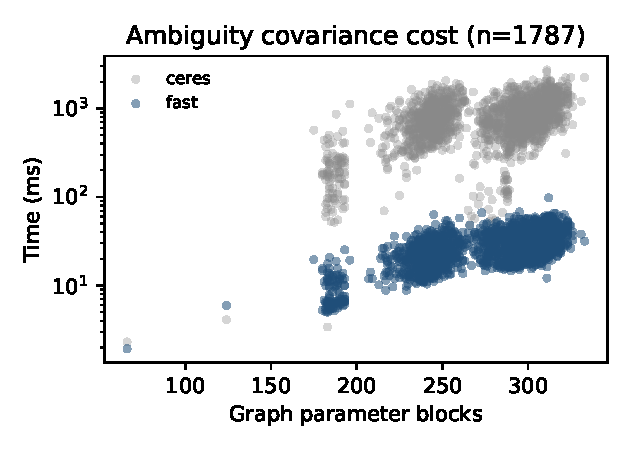
\includegraphics[width=\columnwidth]{F3_timing.pdf}
\caption{Proposed vs.\ Ceres wall time versus graph size (GICI-board~1.1,
$n=1787$).}
\label{fig:timing}
\end{figure}

\paragraph{Complexity.}
Stage~1 is linear in the number of landmarks with $3\times3$ work each.
Stage~2 is cubic in the dense nuisance dimension after landmark elimination,
hence bounded by the sliding window rather than trajectory length---the same
structural reason the method tracks Ceres' marginal while remaining cheaper
than a whole-problem sparse QR each epoch.

%======================================================================
\section{Experimental Setup}
\label{sec:setup}

\begin{table}[!t]
\caption{Datasets}
\label{tab:datasets}
\centering
\scriptsize
\begin{tabular}{@{}p{0.20\columnwidth}p{0.26\columnwidth}p{0.20\columnwidth}p{0.20\columnwidth}@{}}
\toprule
Dataset & Role & DOY & Notes \\
\midrule
GICI-board 1.1 & Cov.\ + runtime & --- & Open-sky \\
UrbanNav Deep & System impact & 141 Whampoa & $n{=}15119$ \\
UrbanNav Med. & Float-path iso.\ (held) & 137 TST & pending isolation \\
\bottomrule
\end{tabular}
\end{table}

UrbanNav Deep uses the session-aligned 5\,s HKKT base slice
\texttt{hkkt141g.21o} (not the full-day 30\,s file).
Primary metric: unaligned raw ENU RMSE (E/N/U, yaw).
Sim(3) APE is used only when comparing to Chi Table~V.
Admissibility: Deep $n_{\mathrm{matched}}\ge14000$; Medium $\ge6500$.
Research flags are opt-in and default-off; the frozen upstream baseline APE on
GICI-board~1.1 ($0.029198$\,m / $0.470557^\circ$, bands $\pm0.005$\,m /
$\pm0.1^\circ$) is re-checked after builds.

Post-file replay is load-sensitive (same Deep sequence spans $\sim$14--24\,min
wall under identical configs).
We treat this as a reproducibility limitation (Sec.~\ref{sec:limits}), not a
scientific contribution; confirmatory UrbanNav numbers below use
identical-load pairing or solo-idle execution.

%======================================================================
\section{Covariance Accuracy and Runtime}
\label{sec:covres}

Open-sky end-to-end with the proposed path preserves accuracy and fix count
inside the frozen band: $0.028991$\,m / $0.4727^\circ$, 869/1775 fixed versus
baseline 876/1775.
Thus, when the measurement model is well behaved, joint $Q_{aa}$ neither
inflates fixing nor loses fixes relative to shadow AR.

The local-conditioning approximation is the critical negative control
(Table~\ref{tab:ablation}): it is real-time but unsafe for AR on Deep.
The proposed path removes that catastrophic horizontal regression while
keeping a large fraction of the fix-rate increase that joint information
enables.

\begin{table}[!t]
\caption{Deep horizontal ablation (raw ENU; one protocol per row)}
\label{tab:ablation}
\centering
\scriptsize
\begin{tabular}{@{}llc@{}}
\toprule
Covariance for AR & Deep $h$ (m) & Fix rate \\
\midrule
Shadow (paired w/ local study) & $2.77{\pm}0.44$ & $\sim$1.3\% \\
Local conditioning (unsafe) & $6.75{\pm}2.98$ & $\sim$17\% \\
Shadow (paired w/ proposed) & $3.03{\pm}0.68$ & 1.7\% \\
Proposed exact-in-window & $3.40{\pm}0.78$ & $8.8{\pm}1.2\%$ \\
Ceres exact (oracle e2e) & --- & pending \\
\bottomrule
\end{tabular}\\[0.2em]
{\scriptsize Spreads are repeat-run variation on one Deep sequence, not
independent scenes. Ceres oracle end-to-end is required before claiming
proposed reproduces Ceres AR.}
\end{table}

%======================================================================
\section{End-to-End AR Evaluation}
\label{sec:e2e}

\paragraph{System impact of the covariance swap.}
Table~\ref{tab:e2e} reports paired Deep runs that differ in the AR covariance
path (proposed vs.\ shadow), under the same protocol wave.
Vertical RMSE and yaw improve in all three repeats; fix rate rises about
fivefold; horizontal RMSE is mixed (worse in 2/3 repeats).
These repeats are \emph{not} independent statistical samples; they measure
run-to-run variation under load-sensitive replay.
Medium is withheld from result tables until float-path isolation passes
(Sec.~\ref{sec:limits}): with 0\% NlFix, continuous trajectories must match
before Deep deltas can be attributed solely to AR.

\begin{table}[!t]
\caption{Deep system impact: proposed $Q_{aa}$ vs.\ shadow (one sequence, 3 repeats)}
\label{tab:e2e}
\centering
\scriptsize
\begin{tabular}{@{}lcccc@{}}
\toprule
Arm & $h$ (m) & $u$ (m) & yaw ($^\circ$) & fix \\
\midrule
Shadow & $3.03{\pm}0.68$ & $2.27{\pm}0.27$ & $1.09{\pm}0.28$ & 1.7\% \\
Proposed & $3.40{\pm}0.78$ & $1.46{\pm}0.21$ & $0.66{\pm}0.07$ & 8.8\% \\
\bottomrule
\end{tabular}
\end{table}

\paragraph{What still needs an oracle.}
The decisive end-to-end claim is that proposed AR decisions and trajectories
match a Ceres-fed AR oracle at much lower covariance cost.
That offline oracle is configured but not yet reported here.
Fig.~\ref{fig:tail} shows only that swapping to joint $Q_{aa}$ can change
fix timing and later horizontal error; it is not a causal proof of
prior poisoning.

\begin{figure}[!t]
\centering
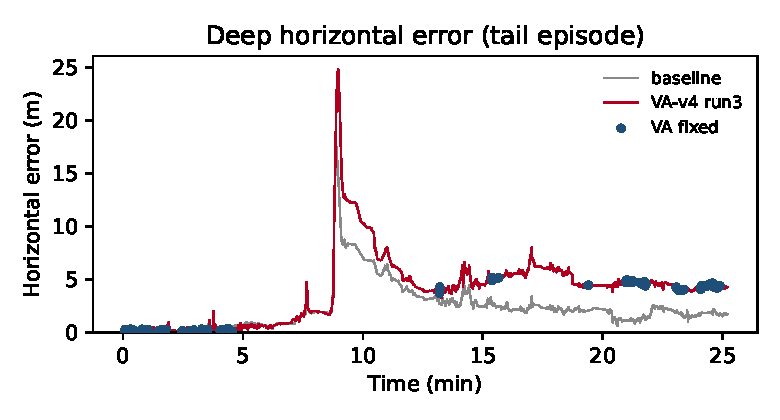
\includegraphics[width=\columnwidth]{F4_tail.pdf}
\caption{Example Deep horizontal error over time (one proposed-path run with a
heavy tail vs.\ a shadow baseline run). Markers: fixed epochs on the proposed arm.}
\label{fig:tail}
\end{figure}

%======================================================================
\section{Limitations}
\label{sec:limits}

\begin{itemize}
\item \emph{Exactness evidence incomplete.} Frobenius match at $10^{-3}$ covers
  90.1\% of usable epochs; Loewner PSD checks, per-diagonal errors, and
  worst-case directional variance ratios are instrumented and must be reported
  before claiming elementwise equivalence to Ceres.
\item \emph{No Ceres e2e oracle yet.} Covariance-level agreement does not imply
  identical AR decisions on UrbanNav; an offline Ceres-fed AR run is required.
\item \emph{Float-path isolation pending.} Arm-to-arm Medium differences at
  0\% NlFix indicate solver-timing / WlFix / ordering confounders until a
  deterministic isolation test passes.
\item \emph{Soft real-time.} The 50\,ms figure is a soft covariance budget at
  $\sim$1\,Hz AR; 4.3\% exceed it (max 97.5\,ms). Report optimize+cov latency.
\item \emph{Statistics.} Three repeats of one Deep sequence are not three
  independent environments.
\item \emph{Decision-layer urban mitigations} are outside this letter.
\end{itemize}

%======================================================================
\section{Conclusion}
\label{sec:concl}

We presented a domain-structured online path to the exact-in-window marginal
ambiguity covariance of a tightly coupled GNSS--IMU--vision factor graph,
with numerical abstention and shadow fallback.
On open-sky graphs it is about 29$\times$ faster than requesting the same
blocks from \texttt{ceres::Covariance}, produces a validated output on 99.94\%
of epochs, and achieves Frobenius relative error below $10^{-3}$ on 90.1\% of
usable epochs.
Stronger Loewner diagnostics, a Ceres end-to-end AR oracle, and float-path
isolation are the remaining measurements needed before submission-strength
exactness and causality claims.
Secondary Deep system effects versus shadow AR (more fixes; mixed horizontal)
must be interpreted in that light.

\section*{Reproducibility}
Opt-in flags, configs, and evaluation scripts are in the accompanying
repository (\texttt{research/paper/README.md}).
Runtime percentiles regenerate from \texttt{[vaar-fast]} logs via
\texttt{scripts/fig\_timing.py}.
Table generation: \texttt{scripts/eval\_paper\_tables.py}.

\balance
\bibliographystyle{IEEEtran}
\bibliography{refs}

\end{document}
